\documentclass[11pt]{amsart}
\usepackage[margin=1in]{geometry}
\usepackage{amsmath,amssymb,amsthm,mathtools}
\usepackage{enumitem,booktabs,array}
\usepackage{tikz}
\usetikzlibrary{calc}
\usepackage[hyphens]{url}
\usepackage[hidelinks]{hyperref}

\newtheorem{theorem}{Theorem}[section]
\newtheorem{lemma}[theorem]{Lemma}
\newtheorem{proposition}[theorem]{Proposition}
\newtheorem{corollary}[theorem]{Corollary}
\theoremstyle{definition}
\newtheorem{definition}[theorem]{Definition}
\theoremstyle{remark}
\newtheorem{remark}[theorem]{Remark}

\newcommand{\I}{\mathrel{\mathrm{I}}}
\newcommand{\nI}{\mathrel{\not\mathrel{\mathrm{I}}}}
\newcommand{\cS}{\mathcal{S}}
\newcommand{\cC}{\mathcal{C}}
\newcommand{\cO}{\mathcal{O}}
\newcommand{\cE}{\mathcal{E}}
\newcommand{\cM}{\mathcal{M}}
\newcommand{\lam}{\lambda}
\newcommand{\PG}{\mathrm{PG}}
\newcommand{\diam}{\operatorname{diam}}
\newcommand{\status}[1]{\textup{[#1]}}

\title[What plays the role of a conic]{What plays the role of a conic: the lab's constructions and ovals, ovoids and polarities}
\author{Degree--diameter lab}
\date{29 October 2026}

\begin{document}
\sloppy\emergencystretch=2em

\begin{abstract}
A sequel to \texttt{SYNTHETIC.md} (branch \texttt{claude/synthetic-incidence-geometry-s4m08f}), written for
Gabriela Araujo-Pardo and Ignacio L\'opez, who asked what happens with conics in generalized polygons. We first say
what a conic is combinatorially (an oval, and the set of absolute points of a polarity) and what plays these two
roles in generalized quadrangles and hexagons. Then we look at each construction of the lab through these objects.
In a projective plane of odd order the answer is sharp: if the frame of the three-hat or four-hat construction is
placed relative to a conic (the special point is the pole of the special line, two marked points are the points of
contact of the tangents from it, and the other two marked points are conjugate), the polarity of the conic extends
to a polarity of the whole structure (Theorem~\ref{thm:selfpolar}). This explains the links and the rotation, gives
an explicit regular completion (the polarity itself), and folds the structure into a graph of diameter~$2$ with
$q^2+q+6$ vertices and maximum degree $q+2$. A conic-adapted choice does not give a fifth hat: every such frame is
infeasible in the hat model for $q\le13$, and no self-polar five-hat extension of $\PG(2,5)$ exists without changing the plane. In quadrangles and
hexagons the conic-like objects (ovoids, partial ovoids, spreads, elliptic quadric sections) are already the
ingredients of Theorems A--D and of the diameter-$7$ freed sets; we restate how, give Theorem~A as a statement
about pairs of conics, and record what the polarity picture gives there. Two lab values are improved: the hexagon
analogues of the conic (the point set of the Hermitian spread, and the lines meeting a spread line together with the
exact whiskers of Theorem~D) are the largest freed sets of the diameter-$7$ construction, and give
$n_b(14,7)\ge1{,}802{,}400$ (lab value $1{,}789{,}588$) and, with a Haar hub graph over $\mathrm{PSL}(2,29)$,
$n_b(15,7)\ge2{,}504{,}544$ (lab value $2{,}501{,}491$).
Every statement is labelled \status{new}, \status{restatement} or \status{standard}, and \status{proof}, \status{computer} or
\status{heuristic}.
\end{abstract}

\maketitle

\setcounter{section}{-1}
\section{Conventions and the dictionary}

We use the conventions of \texttt{SYNTHETIC.md} \S0: an incidence structure has points, lines and a symmetric
incidence~$\I$; its incidence graph has the elements as vertices and the flags as edges; distances and the diameter
are taken there. For the hat constructions we use the frame and the six rules (R1)--(R6) of \texttt{SYNTHETIC.md},
Definition~1.1, with the same names: anti-flag $(A,\ell)$, marked points $X_s$ on $\ell$ ($s\in S$), lines
$\lam_s=AX_s$, a distinguished label $a$, $T=S\setminus\{a\}$, links $\pi$ and rotation $\rho$ (permutations of $T$),
new points $Q,H_s$ and new lines $M,K_s$.

\subsection{What a conic is, combinatorially}
In $\PG(2,q)$ a \emph{conic} $\cC$ is a set of $q+1$ points, no three collinear (an \emph{oval}); for $q$ odd every
oval is a conic (Segre). For $q$ odd a conic is also the set of absolute points ($p\I p^\perp$) of an
\emph{orthogonal polarity} $\perp$: an incidence-preserving involution exchanging points and lines. Both
descriptions have analogues in generalized polygons, and they are different objects there:

\begin{center}\small
\begin{tabular}{@{}p{2.6cm}p{3.4cm}p{4.3cm}p{5.2cm}@{}}
\toprule
& projective plane & generalized quadrangle & generalized hexagon \\
\midrule
``no two too close'' (arc / partial ovoid) & arc: no $3$ collinear; oval: $q+1$ points ($q+2$, hyperoval, $q$ even)
& partial ovoid: pairwise non-collinear; ovoid: $st+1$ points, one on every line
& distance-$2$ (partial) ovoid: non-collinear ($q^4+q^2+1$ points, one on every line; known only for $q=2,3,4$);
distance-$3$ (partial) ovoid: pairwise opposite ($q^3+1$ points) \\
absolute points of a polarity & conic ($q$ odd); a line ($q$ even, pseudo-polarity); Hermitian curve ($q$ square)
& Suzuki--Tits ovoid of $W(q)$, $q=2^{2e+1}$ (the only case with a polarity); absolute lines form a spread
& Ree--Tits ovoid of $H(q)$, $q=3^{2e+1}$ (the only case with a polarity); absolute lines form a spread \\
dual object & dual conic (tangent lines) & spread & spread (Hermitian spread, every $q$) \\
quadric sections & conic $=$ plane section of a quadric
& $Q(4,q)$: elliptic sections $Q^-(3,q)$ are ovoids; plane sections are conics ($q+1$ pairwise non-collinear points)
& $Q(6,q)$: elliptic sections $Q^-(3,q)$ are partial ovoids ($q^2+1$); the lines in an elliptic hyperplane
$Q^-(5,q)$ form a spread (Hermitian spread) \\
\bottomrule
\end{tabular}
\end{center}

\noindent \status{standard} \cite{VM98,PT,Th81,BGS06}. The lab's constructions use the first and third rows
throughout (Sections 2 and 3). The second row, the polarity, is what explains the hats (Section 1).

\subsection{Polarities fold incidence structures}\label{ssec:fold}
A \emph{polarity} of an incidence structure $\cS$ is a bijection $\theta$ from points to lines and lines to points
with $\theta^2=\mathrm{id}$ and $p\I L\iff\theta(L)\I\theta(p)$. A point $p$ is \emph{absolute} if $p\I\theta(p)$.
The \emph{polarity graph} $G_\theta$ has the points of $\cS$ as vertices, $p\sim r$ iff $p\ne r$ and $p\I\theta(r)$
(symmetric because $\theta$ is a polarity). For $\PG(2,q)$ with an orthogonal polarity this is the Erd\H{o}s--R\'enyi
graph.

\begin{lemma}[Folding]\label{lem:fold}
\status{standard; proof} Let $\cS$ have a polarity $\theta$, all degrees at most $\Delta$ and diameter $D\ge2$. Then
$G_\theta$ has maximum degree at most $\Delta$ and diameter at most $D-1$, and $|V(G_\theta)|$ is half the number of
elements of $\cS$.
\end{lemma}
\begin{proof}
The degree of $p$ in $G_\theta$ is the number of lines through $p$, minus one if $p$ is absolute. Map each element
$x$ of a path in the incidence graph to $x$ if it is a point and to $\theta(x)$ if it is a line. Consecutive elements
$u\I L$ go to $u$ and $\theta(L)$, which are equal or adjacent in $G_\theta$ (as $u\I\theta(\theta(L))$). So a path
of length $m$ from $p$ to an element $y$ gives a walk of length at most $m$ from $p$ to $y$ or $\theta(y)$. For points
$p\ne r$, $d(p,r)$ is even and $d(p,\theta(r))$ is odd, both at most $D$; the smaller of the two is at most $D-1$.
\end{proof}

So a self-polar bipartite graph of diameter $D$ gives a graph of diameter $D-1$ with half the vertices. In this
note it is used in two ways: as a description of what the conic does to the hats (\S1.3), and to compare with the
tables of the general degree--diameter problem (where it gives nothing new; \S\S1.3, 2.4, 3.2).

\subsection{Cloning, and why the cloned sets are ovals and ovoids}\label{ssec:clone}
A \emph{clone} of a point $x$ is a new point incident with exactly the lines through $x$; a \emph{line clone} of $L$
is a new line incident with exactly the points of $L$ (\texttt{SYNTHETIC.md} \S2.1 calls the second a shadow line
with all stand-ins original).

\begin{lemma}[Cloning]\label{lem:clone}
\status{standard; proof} Let $\cS$ have diameter $D\ge2$, and add a clone $x'$ for each entry $x$ of a multiset $X$ of
points. Then distances between old elements do not change, $d(x',y)=d(x,y)$ for every element $y\ne x$, and
$d(x',x)=2$; so the diameter is still $D$. A line $L$ gains $|L\cap X|$ incidences (with multiplicity) and no old
point gains any. Dually for line clones; and point clones and line clones may be added together: a clone $x'$ of $x$
and a clone $L'$ of $L$ are at distance at most $d(x,L)$ if $x\nI L$, at most $3$ if $x\I L$, and $1$ if one adds the
flag $x'\I L'$.
\end{lemma}
\begin{proof}
A shortest path from $x$ to $y\ne x$ leaves $x$ along a line through $x$, which also passes through $x'$; conversely
a path from $x'$ is a path from $x$ after its first step. Two clones of one point have a common line.
\end{proof}

So adding points never hurts the diameter; it only costs degree. If every old element may gain $k$ incidences, the
point multisets that can be cloned are exactly those with at most $k$ entries on every line. This is where the
conic-like objects come from \status{restatement}:
\begin{itemize}
\item \emph{projective plane, $k=1$}: any two points are collinear, so only one point can be cloned. The hats of
\S1 are clones of the marked points of one line $\ell$ that \emph{miss} $\ell$ (each $H_s$ is on the $q$ lines through
$X_s$ other than $\ell$); everything else in the construction repairs what missing $\ell$ breaks;
\item \emph{projective plane, $k=2$}: an arc can be cloned; an oval (a conic) and, dually, its tangent lines give
Delorme's construction at $\Delta=q+3$ (\S\ref{ssec:delorme});
\item \emph{generalized quadrangle, $k=1$}: partial ovoids; an ovoid gives a regular result (Theorem~B with weights,
\texttt{SYNTHETIC.md} \S2; \S2 below);
\item \emph{generalized hexagon, $k=1$}: non-collinear sets (partial distance-$2$ ovoids). A distance-$2$ ovoid with
a distance-$2$ spread would give $2(q+2)(q^4+q^2+1)=2N+2(q^4+q^2+1)$ elements at $\Delta=q+2$, fewer than Theorem~D's
$2N+2q^4+4q^3+4q+10$, which doubles along pairwise opposite elements with levels instead.
\end{itemize}
In the plane the conic therefore enters in two different ways: as a set that can be cloned when the degree may rise by
two, and (Section~1) as the absolute set of the polarity that organizes the hats when it may rise by one.

\section{Projective planes: the hats relative to a conic}

\subsection{The conic frame}
Let $q$ be odd, $\cC$ a conic of $\Pi=\PG(2,q)$ and $\perp$ its polarity. A point off $\cC$ is \emph{external}
(on two tangents) or \emph{internal} (on none). We use the following standard facts \status{standard}.

\begin{proposition}[Conjugation on a polar line]\label{prop:conj}
Let $A\notin\cC$ and $\ell=A^\perp$. For a point $X$ of $\ell$, the polar line $X^\perp$ passes through $A$; write
$X^\tau=X^\perp\cap\ell$. Then $\tau$ is an involution of the points of $\ell$ and $X^\perp=AX^\tau$. Its fixed
points are the points of $\ell\cap\cC$: two points $Z,Z'$ if $A$ is external (then $AZ$, $AZ'$ are the two tangents
from $A$, touching $\cC$ at $Z$ and $Z'$), none if $A$ is internal. If $A$ is external, $X^\tau$ is the harmonic
conjugate of $X$ with respect to $Z,Z'$; $X$ and $X^\tau$ are \emph{conjugate} points.
\end{proposition}

So there are two matchings between the points of $\ell$ and the lines through $A$: the frame matching
$X\mapsto AX$, which rule (R1) uses, and the polar matching $X\mapsto X^\perp=AX^\tau$. They differ by $\tau$.
The marked points are now chosen as follows.

\begin{definition}[Conic frame]\label{def:frame}
Let $A$ be external, $\ell=A^\perp$, $\ell\cap\cC=\{Z,Z'\}$, and $X\in\ell\setminus\cC$.
\emph{Three hats:} $(X_a,X_0,X_1)=(Z,X,X^\tau)$. \emph{Four hats:} $(X_a,X_c,X_0,X_1)=(Z,Z',X,X^\tau)$.
In words: $A$ is the pole of $\ell$; the marked points are the two points of contact of the tangents from $A$ (only
one of them for the three hats) and a pair of points of $\ell$ that separates them harmonically. The lines
$\lam_a=AZ$ and $\lam_c=AZ'$ are the tangents from $A$, and $\lam_0=(X^\tau)^\perp$, $\lam_1=X^\perp$.
\end{definition}

\begin{figure}[ht]
\centering
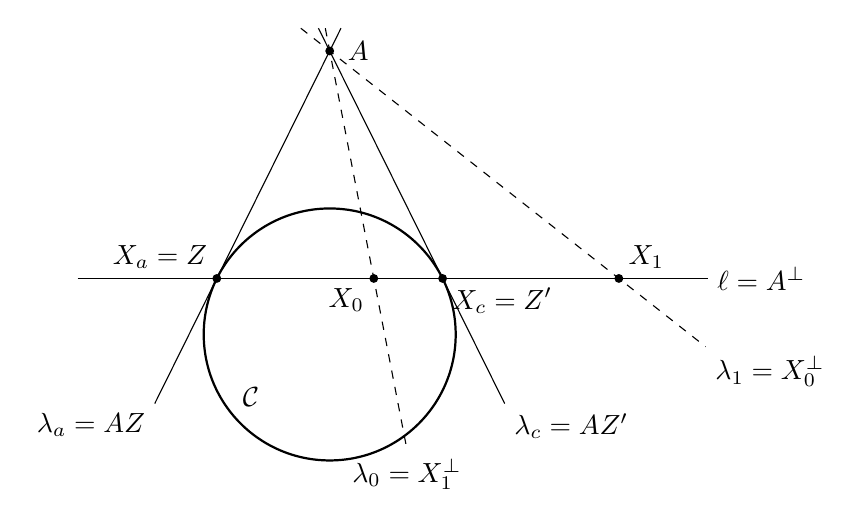
\begin{tikzpicture}[scale=0.8]
  \draw[thick] (0,0) circle (2);
  \node at (-1.25,-1.0) {$\cC$};
  \coordinate (A) at (0,4.5);
  \coordinate (Z) at (-1.792,0.889);
  \coordinate (Zp) at (1.792,0.889);
  \coordinate (X0) at (0.7,0.889);
  \coordinate (X1) at (4.59,0.889);
  \draw (-4,0.889) -- (6,0.889) node[right] {$\ell=A^\perp$};
  \draw ($(A)!-0.1!(Z)$) -- ($(A)!1.55!(Z)$) node[below left] {$\lambda_a=AZ$};
  \draw ($(A)!-0.1!(Zp)$) -- ($(A)!1.55!(Zp)$) node[below right] {$\lambda_c=AZ'$};
  \draw[dashed] ($(A)!-0.1!(X0)$) -- ($(A)!1.75!(X0)$) node[below] {$\lambda_0=X_1^\perp$};
  \draw[dashed] ($(A)!-0.1!(X1)$) -- ($(A)!1.3!(X1)$) node[below right] {$\lambda_1=X_0^\perp$};
  \fill (A) circle (2pt) node[right=3pt] {$A$};
  \fill (Z) circle (2pt) node[above left] {$X_a=Z$};
  \fill (Zp) circle (2pt) node[below right] {$X_c=Z'$};
  \fill (X0) circle (2pt) node[below left] {$X_0$};
  \fill (X1) circle (2pt) node[above right] {$X_1$};
\end{tikzpicture}
\caption{The conic frame of the four hats (drawn over the reals). $A$ is external, $\ell$ is its polar, the chord of
contact $ZZ'$; the marked points are $Z$, $Z'$ and a pair $X_0,X_1$ that separates them harmonically, so that
$AX_0$ is the polar of $X_1$ and $AX_1$ the polar of $X_0$. The three hats use $Z$, $X_0$, $X_1$.}
\label{fig:frame}
\end{figure}

Figure~\ref{fig:frame} shows the frame. For every odd $q\ge3$ such frames exist ($\ell\setminus\cC$ has $q-1\ge2$ points). The cross-ratio
$(X_a,X_c;X_0,X_1)$ of a four-hat conic frame is $-1$; conversely every four-hat frame with $(X_a,X_c;X_0,X_1)=-1$
is a conic frame for each non-degenerate conic of the pencil of conics tangent to $AX_a$ at $X_a$ and to $AX_c$ at $X_c$.
\status{standard}

\subsection{The polarity extends}
Let $\tau$ also denote the permutation of labels with $X_{\tau(s)}=X_s^\tau$; in a conic frame $\tau$ swaps $0$ and
$1$ and fixes $a$ (and $c$). The next lemma is stated for any polarity $\theta$ of a projective plane with
$\theta(A)=\ell$; then $\tau$, defined by $X^\tau=\theta(X)\cap\ell$, is again an involution of $\ell$ whose fixed
points are the absolute points of $\ell$.

\begin{lemma}\label{lem:criterion}
\status{new; proof} Let $\Pi$ be a projective plane with a polarity $\theta$, $A$ a non-absolute point,
$\ell=\theta(A)$, and let the marked set $\{X_s\}$ be $\tau$-invariant. Suppose
$$\tau(a)=a,\qquad \tau\pi\tau=\pi^{-1},\qquad \tau\rho\tau=\rho^{-1}\quad\text{(on $T$)}.$$
Then $\hat\theta$, equal to $\theta$ on $\Pi$ and with $H_s\leftrightarrow K_{\tau(s)}$, $Q\leftrightarrow M$, is a
polarity of the structure $\cS=\cS(\Pi;A,\ell,(X_s),\pi,\rho)$ of \texttt{SYNTHETIC.md}, Definition~1.1.
\end{lemma}

\begin{proof}
$\hat\theta$ is an involution exchanging points and lines; we show that it maps each flag $(p,L)$ of $\cS$ to a
flag $(\hat\theta(L),\hat\theta(p))$. Note $\theta(X_s)=AX_{\tau(s)}=\lam_{\tau(s)}$ and hence
$\theta(\lam_s)=X_{\tau(s)}$.

(R1) $\theta$ maps flags of $\Pi$ to flags of $\Pi$. The deleted flags $(X_s,\lam_s)$ go to
$(\theta(\lam_s),\theta(X_s))=(X_{\tau(s)},\lam_{\tau(s)})$, again deleted. An added flag $(X_t,\lam_{\rho(t)})$ goes
to $(X_{\tau\rho(t)},\lam_{\tau(t)})$; with $u=\tau\rho(t)$ we have $\rho(u)=\rho\tau\rho(t)=\tau(t)$, because
$\tau\rho\tau=\rho^{-1}$ gives $\rho\tau\rho=\tau$. So it is the added flag $(X_u,\lam_{\rho(u)})$.

(R2)$\leftrightarrow$(R3) If $N\I X_s$, $N\ne\ell$, then $\theta(N)$ is a point of $\theta(X_s)=\lam_{\tau(s)}$ other
than $\theta(\ell)=A$, so $(\theta(N),K_{\tau(s)})$ is a flag by (R3). The converse is the same computation.

(R4)$\leftrightarrow$(R5) A point $p\in\ell$ goes to the line $\theta(p)=Ap^\tau$ through $A$. If $p$ is unmarked,
so is $p^\tau$, and $\theta(p)\in\Lambda^*$; $\theta(X_a)=\lam_a\in\Lambda^*$; and $\theta(X_t)=\lam_{\tau(t)}$ with
$\tau(t)\in T$. So $\theta$ maps $\ell^*$ onto $\Lambda^*$, and $(p,M)\mapsto(Q,\theta(p))$ preserves (R4)/(R5).
$(H_s,M)\mapsto(Q,K_{\tau(s)})$.

(R6) $(A,K_a)\mapsto(H_a,\ell)$. A link $(H_t,K_{\pi(t)})$ goes to $(H_{\tau\pi(t)},K_{\tau(t)})$, and with
$u=\tau\pi(t)$, $\pi(u)=\pi\tau\pi(t)=\tau(t)$; so it is the link of $u$.
\end{proof}

\begin{theorem}[Self-polar hats]\label{thm:selfpolar}
\status{new; proof and computer} Let $q$ be odd. In a conic frame (Definition~\ref{def:frame}) the polarity of the
conic, extended by
$$H_a\leftrightarrow K_a,\quad H_c\leftrightarrow K_c,\quad H_0\leftrightarrow K_1,\quad H_1\leftrightarrow K_0,
\quad Q\leftrightarrow M,$$
is a polarity of the three-hat structure of \cite{AL20} and of the four-hat structure.
\end{theorem}

\begin{proof}
Lemma~\ref{lem:criterion} with $\tau=(0\ 1)$. Three hats: $\pi=(0\ 1)$ commutes with $\tau$ and is an involution,
$\rho=\mathrm{id}$. Four hats: $\pi=\rho=\sigma=(0\ c\ 1)$ and $\tau\sigma\tau=(1\ c\ 0)=\sigma^{-1}$.
\end{proof}

\emph{Computer.} \texttt{conics/polar\_frames.py} checks the theorem for every conic frame (every external $A$, every
choice of $Z$, $X$) for $q=3,5,7$, and for random frames at $q=9,11,13$; four independent squad programs
(\texttt{squads/conics-r1/c1}--\texttt{c4}) re-derived it from the rules for $q=3,\dots,13$ and over
$\mathrm{GF}(9)$, $\mathrm{GF}(25)$ (163 instances), and showed for $q=5,7$ that, with $\theta$ and $\tau$ as above,
\emph{exactly} the conic frames are self-polar (2,496 labelled frames tried). The same lemma gives self-polar three
hats for $q$ even: the absolute points of a pseudo-polarity form a line $m$, so $\ell=\theta(A)$ has exactly one
absolute point $X_a$ and $\tau=(0\ 1)$ as before, unless $\ell=m$, in which case every point of $\ell$ is absolute,
$\tau$ is the identity and any three marked points will do. For $q$ square a unitary polarity has $\sqrt q+1$
absolute points on $\ell$, which gives self-polar three and four hats. Checked for $q=4,8,16$ (pseudo) and $q=4,9,16$
(unitary), and independently by squad card \texttt{c8} on every non-absolute $A$ at $q=4,8$ (pseudo) and $q=4,9$
(unitary): 6,830 instances, all self-polar with the right $\tau$ (the card's two ``failures'' are the two
$\ell=m$ cases, where its brief wrongly assumed $\tau\ne\mathrm{id}$).

\begin{remark}[Why the conic frame is forced]\label{rem:forced}
\status{proof} For the four hats, a permutation $\tau$ of $S$ as in Lemma~\ref{lem:criterion} must fix $a$, preserve
$T$ and invert the $3$-cycle $\sigma$; so it is a transposition on $T$ and fixes exactly two labels, $a$ and one
$t\in T$. Hence $X_a$ and $X_t$ are absolute points of $\ell$: for an orthogonal polarity, the two points of contact
of the tangents from $A$. For the three hats, $\tau$ fixes $a$ and either swaps $0,1$ or fixes them; the second needs
three absolute points on $\ell$, impossible for a conic. So among frames with $A$ the pole of $\ell$, the lemma
applies exactly to the frames in which $X_a$ and one $X_t$, $t\in T$, are the two points of contact and the other two
marked points are conjugate, with $\tau$ the transposition of $T$ fixing $t$; Definition~\ref{def:frame} is the case
$t=c$, and the other two cases are the same structure with the labels of $T$ renamed along $\sigma$. (Squad card
\texttt{conics-r2/c4} found these frames too, e.g.\ $X_a=Z'$, $X_0=Z$, $\tau=(c\ 1)$ at $q=5$.) The squad check
above confirms that with $\tau=(0\ 1)$ no other labelled frame is self-polar.

Without fixing $\theta$ the same holds, by a group computation \status{computer}: squad card \texttt{conics-r2/c6}
computed with \texttt{nauty} the full automorphism group of the incidence graph (collineations and correlations) of
the four-hat structure for every cross-ratio $t=(X_a,X_c;X_0,X_1)$ at $q=5,7$. A polarity exists exactly for
$t\in\{-1,2,\tfrac12\}$, i.e.\ exactly when $X_a$ and one point $X_u$, $u\in T$, separate the other two harmonically
(a conic frame up to renaming the labels of $T$, which the $3$-cycle $\sigma$ permits); at $q=7$ the two equianharmonic
frames ($t=3,5$) have no correlation at all and $72$ collineations, against $24$ for the harmonic ones. All
harmonic four-hat structures are isomorphic ($120$ and $336$ labelled harmonic frames at $q=5,7$, one canonical
form), as they must be: the stabilizer of $(A,\ell)$ induces $\mathrm{PGL}(2,q)$ on $\ell$, which is transitive on
harmonic quadruples.
\end{remark}

\subsection{What the gadget is, in polar terms}
Under the polarity every line is $\theta$ of a point, so every incidence $p\I L$ is a symmetric relation
``$p$ is conjugate to $\theta(L)$'' between two points. Reading Table~3 of \texttt{SYNTHETIC.md} this way:

\begin{proposition}\label{prop:gadget}
\status{new; proof} In a four-hat conic frame:
\begin{enumerate}[label=(\alph*)]
\item the four deleted flags $(X_s,\lam_s)=(X_s,X_{\tau(s)}^\perp)$ are exactly the conjugate pairs among the
marked points: $Z$ and $Z'$ with themselves (they are absolute), and $\{X_0,X_1\}$;
\item the three rotation flags $(X_0,\lam_c),(X_c,\lam_1),(X_1,\lam_0)$ make $X_0$ and $Z'$ conjugate (two flags,
$X_0\I Z'^\perp$ and $Z'\I X_0^\perp$) and $X_1$ absolute ($X_1\I X_1^\perp$);
\item the links are the conjugacies $H_0$--$H_c$ (two flags) and $H_1$ absolute, and $A\I K_a$, $H_a\I\ell$ are
the two flags of the conjugacy $A$--$H_a$;
\item $Q$ is conjugate to every $H_s$, to $Z$ and to the unmarked points of $\ell$; $H_s$ is conjugate to the $q$
points of $\lam_{\tau(s)}$ other than $A$ (and $H_a$, by (c), also to $A$).
\end{enumerate}
So the surgery on the old points replaces the conjugacy relation on the marked set
$\{Z,Z',X_0,X_1\}$ (two absolute points and one conjugate pair) by another one (one conjugate pair, $X_0$--$Z'$, and
one absolute point, $X_1$), and the links do the same on the hats.
\end{proposition}
\begin{proof}
(a) $\lam_s=AX_s=\theta(X_{\tau(s)})$. (b) $\lam_c=AZ'=Z'^\perp$, $\lam_1=X_0^\perp$, $\lam_0=X_1^\perp$.
(c) $K_c=\hat\theta(H_c)$, $K_1=\hat\theta(H_0)$, $K_0=\hat\theta(H_1)$, $K_a=\hat\theta(H_a)$, $\ell=\theta(A)$.
(d) $K_s=\hat\theta(H_{\tau(s)})$; $M=\hat\theta(Q)$ contains $\ell^*=\{Z\}\cup\{\text{unmarked}\}$; a line $N\ne\ell$
through $X_s$ is $\theta$ of a point of $\theta(X_s)=\lam_{\tau(s)}$ other than $A$.
\end{proof}

For the three hats in a conic frame the only deleted flag is $(Z,Z^\perp)$ (an absolute point loses its loop),
and the links $H_0\I K_1$, $H_1\I K_0$ make $H_0$ and $H_1$ absolute.

\begin{corollary}[Folding the hats]\label{cor:fold}
\status{new; proof and computer} For every odd prime power $q\ge3$ the polarity graph of the four-hat conic frame is a
graph of diameter $2$ and maximum degree $q+2$ on $q^2+q+6$ vertices; that of the three hats has $q^2+q+5$ vertices.
\end{corollary}
\begin{proof}
Theorem~\ref{thm:selfpolar}, Lemma~\ref{lem:fold} and Theorem~1.7 of \texttt{SYNTHETIC.md} (diameter $3$, degrees
at most $q+2$).
\end{proof}

By Proposition~\ref{prop:gadget}, this graph is the Erd\H{o}s--R\'enyi graph of $\PG(2,q)$ with the edge $X_0X_1$
replaced by $X_0Z'$, plus five vertices: $Q$ joined to $Z$, to the $q-3$ unmarked points of $\ell$ and to the four
hats; $H_s$ joined to the $q$ points of $\lam_{\tau(s)}$ other than $A$; and $H_a$--$A$, $H_0$--$H_c$. (We checked by computer that this
description is exactly the polarity graph, $q=3,\dots,13$: \texttt{conics/folded\_direct.py}.)
\emph{Comparison} \status{computer}: at $q=13$ this is $188$ vertices at $(\Delta,D)=(15,2)$ for general graphs. The
table of the general problem lists $187$ (E.~Canale, 2012) in the UPC table and $190$ (2026) in the current
Wikipedia table, read on 29 October 2026. So the folded four hats lie between the two and are not a record; at
$\Delta=11,13$ ($q=9,11$: $96$ and $138$) they are far below the tabled $106$ and $162$. The three-hat fold at $q=13$
has $187$ vertices, the old tabled value; we do not know how Canale's graph was built.

The four hats can also be built without changing any incidence of the plane (\texttt{research/plus3/plus3.tex},
Proposition ``the four hats without changing the plane''): labels $a,1,2,3$, a $3$-cycle $s=(1\ 2\ 3)$, and the
rotation carried by the hats ($H_i$ also on $AX_{s(i)}$, $K_i$ also through $X_{s^{-1}(i)}$). Its conic frame is
$X_a=Z$, $X_2=Z'$, $\{X_1,X_3\}$ conjugate, with $\tau=(1\ 3)$, which inverts $s$.

\begin{proposition}[Self-polar four hats on an unchanged plane]\label{prop:zero}
\status{new; proof and computer} In this conic frame the zero-change four-hat structure is self-polar, with
$H_x\leftrightarrow K_{\tau(x)}$ and $Q\leftrightarrow M$. Its polarity graph is the Erd\H{o}s--R\'enyi graph of
$\PG(2,q)$, with \emph{no edge changed}, plus five vertices: a graph of diameter $2$ and maximum degree $q+2$ on
$q^2+q+6$ vertices.
\end{proposition}
\begin{proof}
The same check as in Lemma~\ref{lem:criterion}, rule by rule over the table of the cited proposition; the only new
pairs are the extra incidences, and $(H_i,AX_{s(i)})$ goes to $(X_{\tau s(i)},K_{\tau(i)})$, which is the extra
incidence of $K_{\tau(i)}$ because $s^{-1}\tau=\tau s$. No incidence of the plane is changed, so the old part of the
polarity graph is the Erd\H{o}s--R\'enyi graph.
\end{proof}
\emph{Computer.} \texttt{conics/zero\_polar.py}, $q=3,\dots,13$ (polarity, diameter $3$, old part of the fold equal
to the Erd\H{o}s--R\'enyi graph, fold of diameter $2$); independently squad card \texttt{conics-r2/c1}, $42$
instances ($q=3,\dots,13$, every conjugate pair), with $\tau=\mathrm{id}$ failing as a control.

So, in the language of the general problem: \emph{the Erd\H{o}s--R\'enyi graph of $\PG(2,q)$, $q$ odd, has room for
five more vertices at maximum degree $q+2$ and diameter $2$}, and the five vertices are the folded hats. We have not
searched the literature on extensions of polarity graphs; the count $q^2+q+6$ is below the tabled values except at
$\Delta=15$, as said above.

\subsection{An explicit regular version}
In the four-hat structure the elements of degree $q+1$ (the deficient ones) are the points of $\Pi$ off $\ell$,
other than $A$, on the lines $AY$ with $Y$ unmarked, and dually (\texttt{SYNTHETIC.md}, Lemma~1.4). \texttt{SYNTHETIC.md}
completes the structure by any perfect matching of non-incident deficient pairs (K\"onig). The conic gives one.

\begin{proposition}[The polarity completes the hats]\label{prop:complete}
\status{new; proof and computer} In a conic frame (three or four hats), let $p$ be a deficient point. If $p\notin\cC$
put $\mu(p)=p^\perp$; if $p\in\cC$, let $p^*$ be the second point of $\cC$ on the line $Ap$ and put
$\mu(p)=(p^*)^\perp$, the tangent at $p^*$. Then $\mu$ is a bijection from the deficient points onto the deficient
lines with $p\nI\mu(p)$, so adding the flags $(p,\mu(p))$ makes the structure $(q+2)$-regular (still of diameter
$3$). The completed structure is again self-polar.
\end{proposition}
\begin{proof}
Let $p$ be deficient, on $AY$ with $Y\in\ell$ unmarked. $p^\perp$ does not pass through $A$ (as $p\notin\ell$), is not
$\ell$ (as $p\ne A$), and meets $\ell=A^\perp$ in the pole of the line $pA=AY$. By Proposition~\ref{prop:conj},
$AY=(Y^\tau)^\perp$, so this pole is $Y^\tau$. The marked set is $\tau$-invariant, so $Y^\tau$ is unmarked and $p^\perp$ is
deficient. If $p\in\cC$, the line $AY$ is not a tangent (the tangents from $A$ are $AZ$, $AZ'$ and $Z,Z'$ are marked
in the four hats; in the three hats $Z'$ is unmarked, but $AZ'$ meets $\cC$ only in $Z'\in\ell$, which is not
deficient), so $AY$ is a secant and $p^*\ne p$ is deficient too, $p^*\notin\ell$; its tangent $(p^*)^\perp$ meets
$\ell$ in $Y^\tau$ as before and does not contain $p$. The map $p\mapsto p^\perp$ is injective, and on $\cC$ we
composed it with the involution $p\mapsto p^*$ of the deficient points of $\cC$, so $\mu$ is injective; the numbers
of deficient points and lines are equal (\texttt{SYNTHETIC.md}, Lemma~1.4). Self-polarity: $\hat\theta$ maps the added flag $(p,p^\perp)$ to itself and
$(p,(p^*)^\perp)$ to $(p^*,p^\perp)$, the added flag of $p^*$.
\end{proof}

\emph{Computer.} \texttt{conics/polar\_frames.py} for $q=3,\dots,13$, and independently squad card \texttt{c3}
($24$ instances, $q=3,\dots,13$; the number of deficient points on $\cC$ varies with $X$, from $0$ to $12$ at
$q=13$). The same matching also completes the zero-change four hats of Proposition~\ref{prop:zero} (their deficient
elements are again the points off $\ell$, other than $A$, on the lines $AY$, $Y$ unmarked, and dually; checked for
$q=3,\dots,13$ in \texttt{conics/zero\_polar.py}): this gives a $(q+2)$-regular structure of diameter $3$ that
contains $\PG(2,q)$ with every incidence kept, is self-polar, and has every flag given by an explicit rule. In the
folded graph the added flags $(p,p^\perp)$ are loops, so the regular bipartite version does not give a regular graph
of diameter $2$.

\subsection{Does a conic allow more hats?}
\emph{The question in polar terms.} By Corollary~\ref{cor:fold} a self-polar extension of $\PG(2,q)$ by $k$ new
points and $k$ new lines, of maximum degree $q+2$ and diameter $3$, gives an extension of the Erd\H{o}s--R\'enyi
graph by $k$ vertices, of maximum degree $q+2$ and diameter $2$ (not conversely: the structure has diameter $3$ exactly
when any two points of the fold have a common neighbour, an absolute point counting as its own neighbour); the four
hats are $k=5$, and five hats would be $k=6$.

\emph{Heuristic: what the conic cannot change} \status{heuristic}. For large $q$, any extension by a few new elements
is a \emph{copy configuration} (\texttt{research/plus3/plus3.tex}, Theorem 3.4): every new point copies an old point
and every new line an old line, and the line joining two copied points must itself be copied or carry a deleted flag.
A conic offers a second natural set of points to copy, an arc. But $k$ copied points on a conic have $\binom k2$
joining lines (secants), all of which must be copied or broken; on a line the join is one line ($\ell$, copied by
$M$). So collinear marked points are forced, and the conic can only choose \emph{which} points of $\ell$ are marked
and how the gadget is wired. Theorem~\ref{thm:selfpolar} says that the conic chooses them so that the structure is
self-polar; it does not create room for a fifth hat.

\emph{Computer} \status{computer}:
\begin{enumerate}[label=(\roman*)]
\item \emph{Hat model at conic frames} (\texttt{conics/sat\_hatmodel.py}, the model of
\texttt{research/plus2/sat\_gadget.py}: bulk incidences fixed, every incidence of the gadget free, degree $\le q+2$,
diameter $3$). Five hats at $Z$ and two conjugate pairs, and six hats at $Z,Z'$ and two conjugate pairs, one $Q$ and
one $M$: UNSAT for every choice of the pairs, $q=5,7,9,11,13$, with and without imposing self-polarity
($35$ five-hat and $35$ six-hat frames, $140$ runs, each under $4$\,s; \texttt{conics/hatmodel\_conic.out}). The
four-hat conic frame is SAT in all these runs (control).
\item \emph{All self-polar extensions at $q=5$} (\texttt{conics/sat\_polar.py}): new points and new lines tied by the
conic polarity, all incidences of the new elements free, no change to the plane. $k=5$: SAT. $k=6$ (five hats):
UNSAT. The search is split soundly by the orbit of the conic group $\mathrm{PGL}(2,5)$ that contains the point most
often copied (conic point, external, internal) and the number $r$ of lines through it used by one new point;
see \texttt{conics/k6\_q5\_E0.out} for the cases and times. With changes allowed, up to three $\theta$-pairs of deleted flags and two
$\theta$-pairs of added incidences (the budget the self-polar four hats use), only two of the sixteen cases finished
(no new point on two old lines through one point, UNSAT; a new point on all six lines through a point of the conic,
UNSAT in $482$\,s); the others were stopped unfinished (\texttt{conics/k6\_q5\_E3A2.out}).
\end{enumerate}
Earlier work, which this note does not repeat, ruled out five hats in the hat model at default and random frames
for $q=4,\dots,13$, and $+3$ without changes for $q\ge42$ (\texttt{research/plus2/REPORT.md},
\texttt{research/plus3/plus3.tex}).

\subsection{At $\Delta=q+3$ the conic itself is cloned}\label{ssec:delorme}
\status{restatement} Let $q$ be odd, $\cC$ a conic. Clone every point of $\cC$ and every tangent line of $\cC$, and
add the flag (clone of $p$, clone of the tangent at $p$) for each $p\in\cC$. By Lemma~\ref{lem:clone} the diameter
stays $3$. A secant gains two clones, a tangent one, a passant none; dually an external point is on two tangent
clones, a point of $\cC$ on one, an internal point on none; the clones have degree $q+2$. So the maximum degree is
$q+3$ and there are $2(q^2+q+1)+2(q+1)=2(q^2+2q+2)$ elements: $394$ at $q=13$, the 2013 table value at $(16,3)$
(Delorme's construction; \texttt{research/d3d6/REPORT.md}). The lab's $396$ there is not of this kind: it places three
four-hat gadgets on three anti-flags permuted by a Singer subgroup of order $3$ (\texttt{research/d3d6/REPORT.md}).
Could self-polar gadgets for \emph{one} conic do better? At $\Delta=q+3$ every element may gain two incidences. A
gadget in a conic frame $F=\{A,Z,Z',X,X^\tau\}$ raises by one exactly the lines meeting $F$ ($5q-2$ of them) and,
by the polarity, the points whose polars meet $F$; so several such gadgets fit only if no line meets three of their
frames. \status{computer} At $q=13$ no three frames have this property (\texttt{conics/gadgets16.py}, exhaustive over
the $546$ conic frames up to the conic group), so at most two conic-adapted gadgets fit, and the conic does not reach
the value $396$.

\begin{remark}\label{rem:saturated}
\status{new; proof} No hat gadget can be added on top of the conic clones at $\Delta=q+3$: a gadget raises by one the
degree of every point of its line $\ell$ (\texttt{SYNTHETIC.md}, Lemma~1.4: each point of $\ell$ gains $M$, $K_t$ or
the net $+1$ of the rotation), every line of $\PG(2,q)$ contains external points ($q\ge3$), and external points
already have degree $q+3$. The structure is self-polar (clone of $p$ $\leftrightarrow$ clone of the tangent at $p$),
and its fold has $q^2+2q+2$ vertices at $(\Delta,D)=(q+3,2)$: $197$ at $(16,2)$, below the tabled $200$ and $216$.
\end{remark}
\emph{Computer.} \texttt{conics/conic\_clones.py}, $q=3,\dots,13$: $2(q^2+2q+2)$ elements, maximum degree $q+3$,
diameter $3$, a point of degree $q+3$ on every line, self-polar, fold of diameter $2$.

\section{Generalized quadrangles}

\subsection{The analogues}
In a generalized quadrangle of order $(s,t)$:
\begin{itemize}
\item an \emph{ovoid} is a set of $st+1$ pairwise non-collinear points meeting every line once, a \emph{partial
ovoid} a set of pairwise non-collinear points, an \emph{$m$-ovoid} a set meeting every line in $m$ points, and a
\emph{weighted} $m$-ovoid a multiset doing so; dually spreads and covers \status{standard};
\item in $Q(4,q)$ the elliptic quadric sections $Q^-(3,q)$ are ovoids for every $q$ (and every ovoid of
$Q(4,p)$, $p$ prime, is one \cite{BGS06}); a plane section of $Q(4,q)$ that is a conic is a set of $q+1$ pairwise
non-collinear points, the closest analogue of a conic \emph{inside} the quadrangle; in $W(q)$, $q$ odd, there is no
ovoid, and the elliptic quadrics of $\PG(3,q)$ (ovoids of the space, not of $W(q)$) are what the lab uses \status{standard};
\item $W(q)$ has a polarity if and only if $q=2^{2e+1}$; its absolute points form the Suzuki--Tits ovoid and its
absolute lines a spread \cite{VM98} \status{standard}. This is the analogue of ``conic $=$ absolute points''. For $q$ odd
there is none: $W(q)$ and $Q(4,q)$ are dual and not isomorphic.
\end{itemize}

\subsection{Where they appear in Theorems A--C}
\status{restatement} Theorem~B (\texttt{SYNTHETIC.md}, Theorem~2.2) adds clones over a weight $w$ on the points and
shadow lines over a multiset $\cM$ of lines; for a regular result $w$ must be a weighted $(\Delta-s-1)$-ovoid and
$\cM$ a weighted $(\Delta-t-1)$-cover. So the ovoid-like object is exactly the place where clones go, and the
spread-like object where shadow lines go:

\begin{center}\small
\begin{tabular}{@{}p{2.6cm}p{1.75cm}p{3.0cm}p{2.5cm}p{4.45cm}@{}}
\toprule
cells & quadrangle & clones on & shadow lines over & conic-like content \\
\midrule
$(q+1+j,4)$, $q$ even & $W(q)$ & $j\times$ an ovoid & $j\times$ a spread & ovoid (elliptic quadric or Tits) \\
Theorem A: $(11,4)$, $(13,4)$, $(15,4)$ & $\mathrm{AS}(q)$ & $\cE_1\cup\cE_2$ (weighted $2$-ovoid) & none
& two elliptic quadrics; pairs of conics (Prop.~\ref{prop:thmA}) \\
Prop.~C: $(16,4)$ & $W(13)$ & a $2$-ovoid & $2\times$ a spread & union of two elliptic quadrics (Ebert's partition) \\
$(7,4)$: 359 & $Q(4,5)$ & an ovoid ($Q^-(3,5)$) & $21$ lines (four ovoid points on two) & ovoid; $21=q^2-q+1$, Tallini's bound for partial spreads \\
\bottomrule
\end{tabular}
\end{center}

The limits are also conic-like statements: for $q$ odd, $W(q)$ has no ovoid and $Q(4,q)$ no spread, which is why
$\mathrm{AS}(q)$ and weights are used at $\Delta=q+2$; on $Q(4,q)$ with one ovoid of clones the shadow lines form a
partial spread (or nearly), so at most $q^2-q+2$ of them (Tallini's bound $q^2-q+1$ for partial ovoids of $W(q)$,
\texttt{POLISHED.md} Remark~3.5), and the lab's searches found $52,72,92$ at $q=9,11,13$ against the $61,97,141$ needed
to beat Theorem~A (\texttt{research/gq4x/REPORT.md}). Large partial ovoids of $W(3,q)$ in the literature
\cite{CDPS22} are far smaller than this.

\subsection{Theorem A as a statement about pairs of conics}
Theorem~A (\texttt{POLISHED.md} \S4) works in $\PG(3,q)$, $q$ odd, with the symplectic form
$\beta(u,v)=u_0v_1-u_1v_0+u_2v_3-u_3v_2$, the point $x=(1{:}0{:}0{:}0)$, a non-square $\varepsilon$ and the
elliptic quadrics $\cE_1: 2X_0X_1=X_2^2-\varepsilon X_3^2$ and $\cE_2: 2\varepsilon X_0X_1=X_2^2-\varepsilon X_3^2$,
both through $x$ with tangent plane $x^\perp$. The lines of $\mathrm{AS}(q)$ not through $x$ are the totally
isotropic lines $L\not\ni x$ minus their point $z$ in $x^\perp$, and $L$ lies in the plane $z^\perp$, which contains
$x$.

\begin{proposition}\label{prop:thmA}
\status{restatement; proof and computer} For every point $z\ne x$ of $x^\perp$, the plane $z^\perp$ meets $\cE_1$ and
$\cE_2$ in two conics $\cC_1(z),\cC_2(z)$ through $x$ with the same tangent $xz$ at $x$, and from the point $z$ of
this common tangent every other line of $z^\perp$ through $z$ is a secant of one conic and a passant of the other,
or a tangent of both. Equivalently (because every line of $\mathrm{AS}(q)$ of the second kind lies in exactly one
such plane, and the fibres through $x$ meet each quadric once), $\mathbf 1_{\cE_1\setminus x}+\mathbf 1_{\cE_2\setminus x}$
is a weighted $2$-ovoid of $\mathrm{AS}(q)$: this is Theorem~A.
\end{proposition}
\begin{proof}
A plane through $x$ other than $x^\perp$ meets an elliptic quadric through $x$ with tangent plane $x^\perp$ in a
conic through $x$ whose tangent at $x$ is the plane's intersection with $x^\perp$; here that is the line $xz$, as
$x,z\in z^\perp\cap x^\perp$. The lines of $z^\perp$ through $z$ other than $xz$ are the totally isotropic lines
through $z$ not through $x$; the discriminant computation of \texttt{POLISHED.md} (proof of Theorem~4.1) shows that
the line $\ell(a_0,w_0;d)$ meets $\cE_\kappa$ in $1+\chi(\kappa)\chi\bigl(N(d)(a_0-a^*)\bigr)$ points with the same
$a^*$ for both quadrics and $\chi(\kappa_1)=-\chi(\kappa_2)$; this is the secant/passant swap.
\end{proof}

\emph{Computer.} Squad card \texttt{c5} checked (a) both sections are conics through $x$, (b) $xz$ is tangent to both,
(c) the count $2$ and (d) the secant/passant/tangent pattern, for every $z$ at $q=3,5,7,11,13$ ($412$ pairs), for
every non-square $\varepsilon$ ($\varepsilon=1$ fails, as a control), and re-checked the line form of Theorem~A by
enumerating all totally isotropic lines.

So the weighted $2$-ovoid of Theorem~A is a family of \emph{complementary conic pairs}, one pair in each plane
$z^\perp$, all through $x$ and sharing their tangent there; the clone of a point $p\in\cE_i\setminus x$ stands on the
$q+2$ lines through $p$, and every line of $\mathrm{AS}(q)$ gains two clones because each line through $z$ is a secant
of exactly one conic of the pair, or a tangent of both.

\subsection{The polarity picture: $W(2^{2e+1})$}
\begin{proposition}\label{prop:wfold}
\status{restatement; proof} Let $q=2^{2e+1}$, $\theta$ a polarity of $W(q)$, $\cO$ its absolute points (a Suzuki--Tits
ovoid) and $\Sigma$ its absolute lines (a spread). The structure $W(q)[\,j\mathbf 1_\cO,\ j\Sigma\,]$ of Theorem~B
($j$ clones of every point of $\cO$, $j$ shadow lines over every line of $\Sigma$, stand-ins original) is self-polar,
with the $i$-th clone of $p\in\cO$ exchanged with the $i$-th shadow line over $\theta(p)\in\Sigma$. Its polarity graph
has diameter at most $3$, maximum degree $q+1+j$ and $(q+1+j)(q^2+1)$ vertices.
\end{proposition}
\begin{proof}
A flag (clone of $p$, $L$) with $L\ni p$ goes to $(\theta(L),\text{shadow over }\theta(p))$, and $\theta(L)$ lies on
$\theta(p)$; dually for shadow lines. Theorem~B gives diameter $4$ and Lemma~\ref{lem:fold} diameter $3$.
\end{proof}

At $q=8$ this gives $585,650,715$ for $j=0,1,2$, which are the tabled values of the general problem at
$(9,3),(10,3),(11,3)$ (Wikipedia table, read 29 October 2026); we have not checked the provenance of those graphs,
and expect them to be of this kind; for $j=3$ it gives $780<810$. \emph{Computer} (squad card \texttt{conics-r2/c2}): for $q=2$, all $36$ polarities of $W(2)$ were
enumerated with \texttt{nauty}, their absolute points form an ovoid and absolute lines a spread, and for $j=1,2$ the
structure is self-polar of diameter $4$ and folds to $20$ and $25$ vertices of diameter $3$; for $q=8$ a polarity of
$W(8)$ was found in the automorphism group (order $6{,}340{,}239{,}360$) and the folds for $j=1,2$ have $650$ and $715$
vertices, maximum degree $10$ and $11$, diameter $3$. So in quadrangles the polarity picture reproduces
known values and gives nothing at the lab's (odd $q$) cells, where no polarity exists.

\section{Generalized hexagons}

\subsection{The analogues}
\status{standard} In a generalized hexagon of order $(q,q)$ with $N=(q+1)(q^4+q^2+1)$ points: a \emph{distance-$2$
ovoid} is a set of $q^4+q^2+1$ points meeting every line once (pairwise non-collinear; known only for $q=2,3,4$);
a \emph{distance-$3$ ovoid} (an \emph{ovoid}) is a set of $q^3+1$ pairwise opposite points; dually a \emph{spread} is a
set of $q^3+1$ pairwise opposite lines. (A spread in this sense does not partition the points: its lines cover
$(q+1)(q^3+1)$ of the $N$ points, and every other line meets exactly one of them. A set of lines partitioning the points
would be a distance-$2$ spread, with $q^4+q^2+1$ lines.) For the
split Cayley hexagon $H(q)\subset Q(6,q)$, two points are opposite iff they are not orthogonal, so partial ovoids of
$H(q)$ are partial ovoids of the polar space $Q(6,q)$; ovoids exist for $q=3^h$, not for $q$ even \cite{Th81} or $q$
prime $\ge5$ \cite{BGS06}. The \emph{Hermitian spread} (the lines of $H(q)$ in a hyperplane meeting $Q(6,q)$ in an
elliptic $Q^-(5,q)$) exists for every $q$ \cite{Th80}. $H(q)$ has a polarity iff $q=3^{2e+1}$; its absolute points
form the Ree--Tits ovoid and its absolute lines a spread \cite{VM98}. The conic-like partial ovoids are the sections
$Q^-(3,q)$ ($q^2+1$ points, every $q$; their plane sections are conics) and, as found by the lab's squads, unions of
conics through one point with a common tangent there (\S3.3).

\subsection{Theorem D}
\status{restatement} Theorem~D (\texttt{SYNTHETIC.md} \S3) doubles $H(q)$ along levels built from a \emph{spread}
$\Sigma$, one line $v\in\Sigma$ and an exact whisker set. The spread plays the role that the special line plays for
the hats: the components of the doubled set are the ball of radius $2$ about $v$ and one ``broom'' per spread line,
and the ceiling $q|\mathcal A_0|+2(q^3+1)=2N$ is reached because every element outside $\mathcal A_0$ sees exactly one
element of it. For odd $q$ the whiskers come from $q^2-1$ further Hermitian spreads through $v$ (with $\Sigma$, $q^2$
spreads pairwise meeting only in $v$), so the whole configuration is cut out by elliptic hyperplane sections; we
found no conic-level description beyond this. The levels are not invariant under a polarity (they contain spread
lines but not the corresponding ovoid points), so the folding of \S\ref{ssec:fold} does not apply to Theorem~D as it stands.

\emph{A self-polar doubling} \status{new; proof}. For $q=3^{2e+1}$ take the polarity $\theta$, its Ree--Tits ovoid $\cO$
and absolute spread $\Sigma$, and the single level $\mathcal A_0=\cO\cup\Sigma$. Its components are the $q^3+1$ flags
$(p,\theta(p))$ (trees of diameter $1$), a point off $\cO$ is on at most one line of $\Sigma$ and a line off $\Sigma$
has at most one point of $\cO$, so conditions (L0) and (C) of \texttt{SYNTHETIC.md} \S3.1 hold and the doubling with $m$
versions has diameter $6$, maximum degree $q+m$ and $2N+2(m-1)(q^3+1)$ elements. It is self-polar, so it folds to a
graph of diameter $5$ with $N+(m-1)(q^3+1)$ vertices: $392$ at $(5,5)$ for $q=3$, $m=2$, far below the tabled $650$.
Not a record; recorded only because it is the hexagon analogue of Corollary~\ref{cor:fold}. \emph{Computer} (squad card
\texttt{conics-r2/c3}): $H(3)$ built from Tits' equations; a polarity found with \texttt{nauty} (the automorphism group
of the incidence graph has order $8{,}491{,}392=2|G_2(3)|$); its $28$ absolute points are pairwise opposite, its $28$
absolute lines pairwise opposite, each absolute point on one absolute line; the doubling has $784$ elements, maximum
degree $5$, diameter $6$, is self-polar, and folds to $392$ vertices of diameter $5$.

\subsection{The diameter-7 freed sets}
\status{restatement, with one squad computation} The diameter-$7$ constructions (\texttt{SYNTHETIC.md} \S4) free the
incidences of a matching at a set $R$ of points. When the matching is a duality ($q=3^h$) or the identity of a friendly
transition (a copy of $H(q)$ followed by a copy of its dual, any $q$), any segment set may be freed, and the point
set of a spread (Hermitian, or the Ree--Tits spread when $q=3^{2e+1}$) is the largest one; with other matchings
$R$ must be non-collinear and the matching a local duality, which is easy when $R$ is a partial ovoid. So the
size of the records at $(7,7),(9,7),(10,7),(13,7)$ is governed by large partial ovoids of $H(q)$, i.e.\ of $Q(6,q)$.
The conic-like ones are:
\begin{itemize}
\item the $q^2+1$ points of an elliptic section $Q^-(3,q)$ (\texttt{D7\_HEXAGON.md}, Corollary~9.1, every $q$);
\item \emph{conic fans}: a point $e$ and $k$ conics through $e$ whose planes share one tangent line at $e$, $1+qk$
points; the points opposite $e$ form an affine space $\mathrm{AG}(5,q)$ in which opposition is $Q'(x-x')\ne0$ for a
quadratic form $Q'$, and each conic is an affine line with non-square $Q'$-direction (\texttt{research/d13D7/REPORT.md}
\S3, $1+11\cdot29=320$ at $q=11$);
\item the record sets themselves (72, 288, 217 and 756 pairwise opposite points at $q=5,7,8,11$, plus a few
mirrored points) come from searches and, at $q=7,11$, from orbits of the Weyl group $W(E_7)$.
\end{itemize}
\emph{Squad computation} \status{computer}: card \texttt{c7} rebuilt the conic fans for $q=5,7$ (direct check of
opposition on all pairs; the $q+1$ points of each fan line with $e$ form a conic of a plane) and searched for large
fans with one direction: at $q=5$ the compatibility graph on the $625$ cosets has clique number exactly $7$ (exact
branch and bound, confirmed by SAT, for every one of the $300$ non-square directions), so single-direction fans have
at most $1+5\cdot7=36$ points; at $q=7$ a tabu search found $15$ lines, $106$ points. The records use $72$ and $288$
pairwise opposite points at these $q$, so at small $q$ the conic fans are not competitive; they become useful only at
$q=11$ (320 points), and there the record set (756) is a Weyl-group orbit, not a fan.

\emph{What the hexagon offers that the plane does not} \status{heuristic}. In the plane the conic's polarity is what
makes the hats self-polar; in the hexagon a polarity exists only for $q=3^{2e+1}$, outside the lab's cells (which
use $q=5,7,8,9,11,13$), and the diameter-$7$ layouts with an odd number of copies are self-polar only if one copy is
mapped to itself, which needs such a polarity. So the conic-as-polarity picture does not reach the hexagon records,
and the conic-as-ovoid picture is already what the records use; \S\ref{ssec:d14} shows that taking these sets as large
as the theory allows improves two of them.

\subsection{Spread points and whiskers as freed sets: $(14,7)\ge1{,}802{,}400$}\label{ssec:d14}
\status{new; proof and computer} The $(14,7)$ record (\texttt{research/cell147/typedmirror/}; $q=11$, $\Delta=q+3$)
takes five copies of the incidence graph of $H(11)$ of types $H$, $H^D$, $H$, $H^D$, $H$ (a copy of $H^D$ is a copy of
$H$ with points and lines renamed), joins each copy to the next two by bijections from its points to their lines, uses
the identity on the six \emph{friendly} transitions (between a copy of $H$ and a copy of $H^D$) and the mirrored local
duality on $768$ points on the four others, and adds hubs (\texttt{SYNTHETIC.md} \S4). On a friendly transition from
$H$ to $H^D$ any segment set $R_H$ of points may be freed, and on one from $H^D$ to $H$ any dual segment set $R_L$ of
lines (Theorem~B of \texttt{D7\_HEXAGON.md}). Every hub takes one freed slot in every copy, so the number of hubs per
side is the smallest number of free slots of a copy; in this layout it is $\min(|R_H|,|R_L|)+768$. The record used a
non-collinear $R_H$ ($8{,}645$ points) and a non-concurrent $R_L$ ($8{,}246$ lines).

The conic-like sets of \S3.1 are the largest freed sets of this kind:
\begin{itemize}
\item $R_H$: the point set of the Hermitian spread $S$ (the lines of $H(11)$ in the elliptic hyperplane $\Pi$:
$x_0+x_4=0$), $(q+1)(q^3+1)=15{,}984$ points, the largest segment set (\texttt{D7\_HEXAGON.md}, Proposition~1.4).
\texttt{D7\_HEXAGON.md}, Remark~9.4, proposed this set, with $R_L$ the $12\cdot756$ lines through a $756$-point partial
ovoid, for $1{,}791{,}240$ elements; it was not built.
\item $R_L$: the lines meeting a fixed line $v\in S$, other than $v$, together with an exact whisker set $W$ of
Theorem~D relative to $S$ and $v$ (\texttt{SYNTHETIC.md} \S3.2; the explicit $W$ of \texttt{POLISHED.md}, Theorem~6.5).
\end{itemize}

\begin{lemma}\label{lem:whiskRL}
\status{new; proof} Let $S$ be a spread of a generalized hexagon of order $(q,q)$, $\mathcal P_S$ its point set,
$v\in S$, and $W$ a whisker set (lines opposite $v$, not in $S$, no point off $\mathcal P_S$ at distance $5$ from $v$
on two of them). Then the lines meeting $v$ other than $v$, together with $W$, form a dual segment set, of size
$q(q+1)+|W|$; for an exact $W$ this is $q(q+1)(q^2-q+1)$.
\end{lemma}
\begin{proof}
Every line $L$ of the set has exactly one point in $\mathcal P_S$: a line meeting $v$ meets no other line of $S$ (its
points other than the one on $v$ are at distance $3$ from $v$, while the points of the other spread lines are at
distance $5$), and a whisker meets exactly one line of $S$ (every line not in $S$ does) once. Its other $q$ points are
at distance $3$ from $v$ (lines meeting $v$) or are free points at distance $5$ (whiskers). A point at distance $3$
from $v$ is on only one line meeting $v$ (two would close a circuit of length $6$, and the girth is $12$), and a free point is on at
most one whisker. So two lines of the set meet, if at all, in their points of $\mathcal P_S$, and all lines of the set
meeting $L$ pass through the one point of $L$ in $\mathcal P_S$. The count is $q(q+1)+q^2(q^2-1)$ for an exact $W$.
\end{proof}

At $q=11$ this gives $|R_L|=14{,}652$, against the bound $(q+1)(q^3+1)=15{,}984$ (reached only by the pencils of an
ovoid, which $H(11)$ does not have). The free slots per copy are then $16{,}752,\ 15{,}420,\ 16{,}752,\ 29{,}304,\
16{,}752$ (outgoing) and $15{,}420,\ 31{,}968,\ 15{,}420,\ 16{,}752,\ 15{,}420$ (incoming), so there are $15{,}420$ hubs per
side, joined by $9$ random perfect matchings (all same-side hub distances at most $6$), and
$$n_b(14,7)\ \ge\ 10\cdot177{,}156+2\,(14{,}652+768)\ =\ 1{,}802{,}400,$$
$12{,}812$ more than the lab's $1{,}789{,}588$ and $30{,}840$ more than the 2013 table ($1{,}771{,}560$).
\emph{Computer.} \texttt{conics/d14D7/tm\_build\_herm.py} (the lab's \texttt{tm\_build.py} with these two sets
computed inside, and segment and dual segment checks in place of the non-collinear and non-concurrent ones) re-checks
every hypothesis: $R_H$ a segment set, $R_L$ a dual segment set, the exact whisker set (every free point on exactly one
whisker), the mirrored set ($768$ points, local duality at each), the hub distances and the degrees ($\le14$); the stored
solution \texttt{research/frontier/sols/d14D7\_hex11\_typedwhisk\_n1802400.sol} rebuilds a byte-identical edge list.
\emph{All-pairs check} (\texttt{apsp\_mt}, every vertex, diameter $\le7$): running at the time of writing; the result goes to \texttt{conics/d14D7/checks/}.

\emph{The same sets at $(15,7)$} \status{new; computer}. The $(15,7)$ layout of the lab's earlier candidate
(\texttt{research/cell147/typedmirror/README.md}: seven copies of types $H,H,H^D,H,H,H^D,H^D$, three matchings per
copy, the mirrored surgery on the nine non-friendly transitions) runs through the same builder. With the two sets above
the tightest copies have $17{,}520$ free outgoing and $16{,}188$ free incoming slots. The hub graph may now have degree
only $15-7=8$, and a random one on $16{,}188$ hubs per side leaves $110{,}476$ same-side pairs at distance more than $6$.
We take instead a Haar graph: hubs on both sides indexed by a group $G$, line-side hub $x$ joined to point-side hub $xs$
for $s$ in a set $S$ of $8$ elements; same-side distances are at most $6$ exactly when $(SS^{-1})^3=(S^{-1}S)^3=G$.
For $G=\mathrm{PSL}(2,29)$ ($12{,}180$ elements) a short local search finds such an $S$
(\texttt{conics/d15D7/psl\_hubgraph2.py}); for $\mathrm{PSL}(2,31)$ ($14{,}880$ elements) it reached $14{,}879$ of
$14{,}880$ and stopped there, also with moves aimed at the missing element (a Haar graph of degree $8$ has
$8\cdot7^5=134{,}456$ non-backtracking paths of length $6$ from a hub, about $9$ per element of $\mathrm{PSL}(2,31)$). With $\mathrm{PSL}(2,29)$,
$$n_b(15,7)\ \ge\ 14\cdot177{,}156+2\cdot12{,}180\ =\ 2{,}504{,}544,$$
against the lab's $2{,}501{,}491$ (table $2{,}480{,}184$); the slots allow up to $2{,}480{,}184+17{,}520+16{,}188=2{,}513{,}892$ (unequal sides) with a better hub graph. No other order of the copy types does better: with these freed sets and
the $768$-point surgery, the largest sum of the smallest outgoing and the smallest incoming free count over all $2^7$
type patterns of seven copies is $17{,}520+16{,}188$ (direct count; in every pattern some copy has at most one copy of
the other type among the three it maps to).
\emph{All-pairs check} (\texttt{apsp\_mt}, every vertex, diameter $\le7$): queued after the $(14,7)$ check; the result goes to \texttt{conics/d15D7/checks/}.

\emph{And at $(16,7)$} \status{computer, not built}. In the same five-copy layout at $q=13$ (record
$4{,}052{,}108=10\cdot402{,}234+2\cdot14{,}884$, with $\min(|R_H|,|R_L|)=14{,}762$ and $122$ elements of surgery on the
non-friendly transitions) the Hermitian spread ($30{,}772$ points) and the exact whiskers ($c=2$, $(c_0,c_1)=(1,1)$ in
\texttt{POLISHED.md}; $|R_L|=13\cdot14\cdot157=28{,}574$) would give $28{,}696$ hubs per side and
$4{,}022{,}340+57{,}392=4{,}079{,}732$, if a hub graph of degree $11$ with same-side distances at most $6$ is found.
We did not build it: the record was checked with an automorphism of order $61$, the new sets are not invariant under
it, and the largest symmetry we found that preserves them (a torus of order $12$ in $G_2(13)$, which fixes $v$) cannot
be extended to the non-friendly transitions (it has $42$ fixed points but only $30$ fixed lines, so no bijection from
points to lines commutes with it); a check without symmetry takes about $5$ times the $(14,7)$ one.

\section{Summary: what is new}\label{sec:summary}
\begin{itemize}
\item \textbf{The role of a conic, in one sentence.} Adding points never hurts the diameter, only the degree
(Lemma~\ref{lem:clone}); so the sets that can be copied are those with few points on every line: ovals in a plane when
the degree may rise by two (Delorme's $(16,3)$ value), ovoids and partial ovoids in quadrangles (Theorems A--C),
non-collinear sets and pairwise opposite sets in hexagons (Theorem~D, the $D=7$ freed sets). When the degree may rise by
only one, a plane allows no such set, and the conic enters instead through its polarity, which organizes the hats.
\item \textbf{New, with proofs and computer checks.} The conic frame of the hats (Definition~\ref{def:frame}); the
three and four hats in a conic frame are self-polar (Lemma~\ref{lem:criterion}, Theorem~\ref{thm:selfpolar}); with
nauty, at $q=5,7$ a four-hat structure has a polarity exactly when its frame is a conic frame up to renaming labels
(Remark~\ref{rem:forced}); the gadget read as a change of the conjugacy relation (Proposition~\ref{prop:gadget}); the
zero-change four hats are self-polar too (Proposition~\ref{prop:zero}); the polarity gives an explicit regular completion
of both (Proposition~\ref{prop:complete}); folding gives graphs of diameter $2$, $q^2+q+6$ vertices, maximum degree
$q+2$, the Erd\H{o}s--R\'enyi graph plus five vertices (Corollary~\ref{cor:fold}); the self-polar doubling of
$H(3^{2e+1})$ (\S3.2); lines meeting a spread line plus whiskers form a dual segment set (Lemma~\ref{lem:whiskRL}).
\item \textbf{New, by computer.} No five or six hats in the hat model at any conic frame for $q\le13$ ($140$ runs); no
self-polar five-hat extension of $\PG(2,5)$ without changes to the plane (every orbit case); at most two
conic-adapted gadgets fit at $\Delta=16$, $q=13$.
\item \textbf{Restatements.} The dictionary of \S0; Theorem~A as complementary conic pairs (Proposition~\ref{prop:thmA});
where ovoids, partial ovoids and spreads sit in Theorems A--D and the $D=7$ freed sets; the $W(8)$ polarity values
(Proposition~\ref{prop:wfold}); Delorme's conic clones at $(16,3)$.
\item \textbf{Lab values.} $(14,7)$: $1{,}802{,}400$ (lab $1{,}789{,}588$), with the Hermitian spread points and the
lines meeting a spread line plus exact whiskers as friendly freed sets (\S\ref{ssec:d14}); all-pairs check: running at the time of writing; the result goes to \texttt{conics/d14D7/checks/}.
$(15,7)$: $2{,}504{,}544$ (lab $2{,}501{,}491$), the same sets in the seven-copy layout with a Haar hub graph over
$\mathrm{PSL}(2,29)$; all-pairs check: queued after the $(14,7)$ check; the result goes to \texttt{conics/d15D7/checks/}. Candidate for the coordinator: $(16,7)$ $4{,}079{,}732$ by the same sets (not built). Nothing else improved; the
folded graphs are below the current tables of the general problem.
\end{itemize}

\appendix
\section{Files and checks}
In \texttt{research/synthetic/conics/}: \texttt{pg2.py} ($\PG(2,q)$, the conic, the hat rules); \texttt{selfpolar.py},
\texttt{polar\_frames.py}, \texttt{folded\_direct.py}, \texttt{pseudo\_absline.py}, \texttt{zero\_polar.py}
(Theorem~\ref{thm:selfpolar}, Corollary~\ref{cor:fold}, Propositions~\ref{prop:zero} and \ref{prop:complete}, all
polarity types); \texttt{conic\_clones.py} (\S\ref{ssec:delorme}); \texttt{sat\_hatmodel.py}, \texttt{run\_hatmodel.py}
(hat model at conic frames); \texttt{sat\_polar.py}, \texttt{run\_cases.sh} (self-polar extensions; \texttt{k6\_q5\_E0.out}
and, partial, \texttt{k6\_q5\_E3A2.out}); \texttt{gadgets16.py} (several conic gadgets at $\Delta=16$);
\texttt{d14D7/} (the $(14,7)$ builder, the exact whisker set, the checks; README there); \texttt{d15D7/} (the
$\mathrm{PSL}(2,29)$ hub graph search and hub graph for $(15,7)$, the check; README there); \texttt{d16D7/hexsets.py}
(the sets of $H(13)$ and their orbit counts under the torus, \S\ref{ssec:d14}). Every script writes its output to
a \texttt{.out} file of the same name. Squad rounds \texttt{research/squads/conics-r1/} and \texttt{conics-r2/} (briefs,
cards, scoreboards), logged in \texttt{research/squads/LOG.md}. Python with \texttt{python-sat} (CaDiCaL 1.5.3) and
\texttt{pynauty}; the all-pairs check is \texttt{research/lifts/coordinator\_check/apsp\_mt.c}.

\begin{thebibliography}{99}
\bibitem{AL20} G. Araujo-Pardo and N. L\'opez, On new record graphs close to bipartite Moore graphs, Graphs Combin.
\textbf{38} (2022), Paper 110; arXiv:2005.02427.
\bibitem{BGS06} S. Ball, P. Govaerts, L. Storme, On ovoids of parabolic quadrics, Des. Codes Cryptogr. \textbf{38}
(2006) 131--145.
\bibitem{CDPS22} M. Ceria, J. De Beule, F. Pavese, V. Smaldore, On large partial ovoids of symplectic and Hermitian
polar spaces, J. Combin. Des. \textbf{31} (2023) 5--22; arXiv:2203.04553.
\bibitem{PT} S. E. Payne and J. A. Thas, Finite Generalized Quadrangles, 2nd ed., EMS, 2009.
\bibitem{Th80} J. A. Thas, Polar spaces, generalized hexagons and perfect codes, J. Combin. Theory Ser. A \textbf{29}
(1980) 87--93.
\bibitem{Th81} J. A. Thas, Ovoids and spreads of finite classical polar spaces, Geom. Dedicata \textbf{10} (1981)
135--143.
\bibitem{VM98} H. Van Maldeghem, Generalized Polygons, Birkh\"auser, 1998.
\end{thebibliography}

\end{document}
